\chapter{Modelado de sistemas dinámicos}
Warning: Section in progress
\section{Ejemplos}
\subsection{Un vehículo de cuatro ruedas. }
La figura \ref{f1} muestra un esquema de un vehículo terrestre de cuatro ruedas, visto desde arriba. Si consideramos que se mueve en el plano $x,y$, y que su velocidad instántanea $\vec{V}$ está siempre orientada en la dirección de avance del vehículo $psi$--asumimos que no derrapa, ni se mueve lateralmente--, podemos entoces definir el velocidad, en el sistema de referencia $x,y$ como,
\begin{align}
\dot{x} = V_x(t) = V\cos(\psi(t))\\
\dot{y} = V_y(t) = V\sin(\psi(t))\\
\end{align}

\begin{figure}
\centering

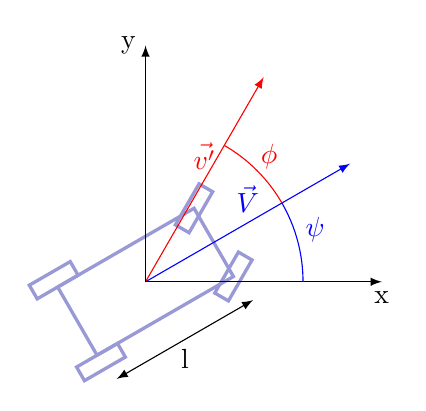
\begin{tikzpicture}
\draw(0,0)[rotate around={30:(0,0)},very thick,draw = blue!60!black!40]rectangle(2,1);
\draw(-0.3,-0.2)[rotate around={30:(0,0)},very thick,draw = blue!60!black!40]rectangle(0.3,0.0);
\draw(-0.3,1)[rotate around={30:(0,0)},very thick,draw = blue!60!black!40]rectangle(0.3,1.2);
\draw({2*cos(30)-0.3},{2*sin(30)-0.1})[rotate around={60:({2*cos(30)},{2*sin(30)})},very thick,draw = blue!60!black!40]rectangle({2*cos(30)+0.3},{2*sin(30)+0.1});
\draw({2*cos(30)-sin(30)-0.3},{2*sin(30)+cos(30)-0.1})[rotate around={60:({2*cos(30)-sin(30)},{2*sin(30)+cos(30)})},very thick,draw = blue!60!black!40]rectangle({2*cos(30)-sin(30)+0.3},{2*sin(30)+cos(30)+0.1});
\draw[blue]({cos(30)-0.5*sin(30)},{sin(30)+0.5*cos(30)})--node[above]{$\vec{V}$}({4*cos(30)-0.5*sin(30)},{4*sin(30)+0.5*cos(30)})[-latex];
\draw[red]({cos(30)-0.5*sin(30)},{sin(30)+0.5*cos(30)})--node[above]{$\vec{v'}$}({cos(30)-0.5*sin(30)+3*cos(60},{sin(30)+0.5*cos(30)+3*sin(60})[-latex];

\draw({cos(30)-0.5*sin(30)},{sin(30)+0.5*cos(30)})--({3+cos(30)-0.5*sin(30)},{sin(30)+0.5*cos(30)})[-latex]node[anchor=north]{x};
\draw({cos(30)-0.5*sin(30)},{sin(30)+0.5*cos(30)})--({cos(30)-0.5*sin(30)},{3+sin(30)+0.5*cos(30)})[-latex]node[anchor=east]{y};

\draw[blue]({2+cos(30)-0.5*sin(30)},{sin(30)+0.5*cos(30)})arc(0:30:2);
\draw[red]({3*cos(30)-0.5*sin(30)},{3*sin(30)+0.5*cos(30)})arc(30:60:2);
\draw[blue]({3.2*cos(30)},{3.2*sin(30)}) node[]{$\psi$};
\draw[red]({3.4*cos(50)},{3.3*sin(50)}) node[]{$\phi$};
\draw[latex-latex](0.25,-0.3)--node[below]{l}({2*cos(30)+0.25},{2*sin(30)-0.3});
\end{tikzpicture}
\label{f1}
\caption{Esquema de un vehículo terrestre de 4 ruedas}
\end{figure}

Además el vehículo girará, siempre que las ruedas delanteras no estén alineadas con las ruedas traseras, cambiando así su dirección de avance . Podemos relacionar la velocidad de giro del vehículo $\dot{\psi}$ con el ángulo de orientación de las ruedas delanteras $\phi$, y la velocidad a la que avanzan $\vec{v'}$.  podemos obtener las componetes de dicha velocidad en ejes cuerpo (paralela y perpendicular a la dirección de avance del vehículo),

\begin{align}
v_{P} = v'\cos(\phi(t))\\
v_{T} = v'\sin(\phi(t))
\end{align} 

Pero la rueda esta unida al vehículo así que su velocidad en la direccíon de avance debe ser la misma que la vel vehículo: $v_P \equiv V$.  A partir de esta relación podemos obtener la velocidad tangencial de las ruedas como,
\begin{equation}
v_T = V\frac{\sin(\phi)}{\cos(\phi)} = V\tan(\phi)
\end{equation}

Si tomamos como centro de giro del vehículo el centro de su eje trasero y la batalla (distancia entre ejes) es $l$, obtenemos una expresión para su velocidad de giro,
\begin{equation}
\dot{\psi} = \frac{V}{l}\tan(\phi)
\end{equation} 
 